% !TEX root = SocialVision2014.tex
\pagestyle{plain} \pagenumbering{arabic}

\Section{Introduction} \label{sec:intro}


Image and video collections contain rich information about human interactions, human relationships, and social structure. Whether it is a personal collection, a shared collection of an online community, or a collection from a surveillance network, any large set of visual observations of people over an extended period of time provides access to co-occurrence counts, relative face and body positions, gestures, expressions, and scene types, all of which provide information about identities, attributes, interactions, and relationships. This social information is richer and more nuanced than that from textual signals like email logs, phone logs, and textual social media, and it will undoubtedly be useful for machines, just as it is useful for humans when analyzing individuals within a social group from a distance; when deciding which colleagues to approach to enact policy changes; or when judging whether to alert authorities of a questionable interaction between strangers: If we had good tools for analyzing behaviors and relationships in large image and video collections, we could build better tools for discovering interaction patterns and social structures in active classrooms, sports matches, and other public spaces. We could also build better human-computer interfaces, recommendation systems, video indexing methods, and security systems.
 
This project will develop a foundation for these applications by introducing image and signal processing paradigms that recognize interactions and extract social information from large-scale imagery: They will extract, from images and videos of human gatherings,  information about the types and frequencies of social interactions that occur; and they will compute useful information about the social network, represented as a social graph that embeds the individuals, groups, and communities, and that encodes the relationships between the individuals as signals on the social graph.  This research will introduce images and video as a new source for ``sensing" a social network and estimating the signals on the social graph, one that complements emails, phone logs, and web-based media by exploiting face positions, body poses, movements, and scene and event types --- things that are critical for analyzing interactions and relationships, but difficult to observe by any other means than from images.


We will achieve our goals by coordinated innovations in two areas: \emph{semantic image processing} and \emph{multidimensional signal processing on (social) graphs}, as shown in Figure~\ref{fig:intro} . For the former, we will exploit the fact that social interactions between two or more people can be broken down into basic spatial and spatio-temporal visual elements; that these visual elements can be usefully categorized; and that the frequency and structure of occurrences of these elemental categories carry information about actors' roles and relationships. These ideas are rooted deeply in anthropological and sociological studies of non-verbal communication, and in this proposal, we borrow and broaden the anthropological term \emph{proxemes} to refer to the basic elements of social interactions. For us, a proxeme can be a relative spatial arrangement of two or more people at a particular instance of time (static; observable in an image), or a space-time sequence of such arrangements (dynamic; observable in a video), and we will develop semantic image processing tools that detect, recognize, and summarize the spatio-temporal occurrences of the proxemes in image and video collections.

For the latter, we will develop new foundations of graph signal processing that transform the social relationship information carried by the proxemes and by other social attributes (e.g., gender, age, and occupation, etc.) to the social network embedding the individuals. Representing a social network as a graph (cell complex) whose nodes (0-cells) correspond to the individuals occurring in the imagery, we are interested in inferring the type of social relationship, among a dictionary of multiple social relationship types/categories (such as parent-child, friends, partners, etc.), for every edge (1-cell), and therefore require models for multi-dimensional, or vector-valued, signals defined on edges. In particular, several challenges combine to make this problem distinctive: 1) proxemes must be inferred from imagery and are therefore very noisy and ambiguous; 2) there is ambiguity in who is interacting because actor identities must also be inferred; and 3) like other network-inference problems, community structures exist at multiple scales and among higher-order cells, and measurements are incomplete because of unobserved co-occurrences.

\begin{figure}[t!]
\begin{center}
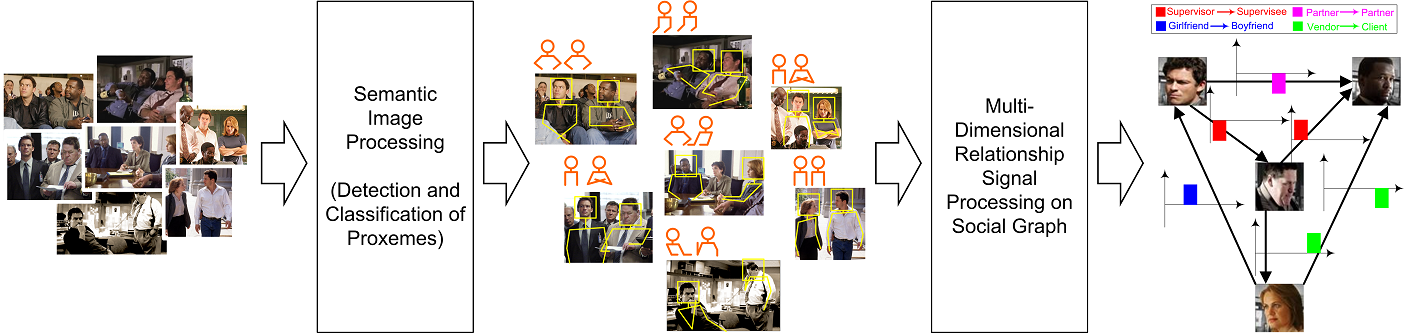
\includegraphics[width=\columnwidth]{overview}
\end{center}
\vspace{-0.25in} \caption{\captionsize 
Social visual analytics: A computational foundation for recovering social relationships and social networks from image and video collections. It contains two mutually coordinated major components: semantic image processing with a focus on detection and classification of proxemes, and multi-dimensional relationship signal processing on social graphs.  Details about the two components are illustrated in Figures~\ref{fig:proxeme_det_recog} and~\ref{fig:SP_on_Graph} respectively.\label{fig:intro}\afterfigspace}
\end{figure}


With these considerations in mind, our project can be described in four parts:


\begin{enumerate}

\vspace{-0.1in}\item \emph{Representing, detecting, and recognizing social proxemes.} We will develop efficient computational representations for the basic elements of social interactions, comprised of mixed ensembles of per-actor descriptors and relative, between-actor descriptors. Along with these, we will co-develop processes for measuring the similarity between two interaction elements, thereby enabling learning of proxeme vocabularies from annotated data, as well as the detection and recognition of proxeme occurrences in large image and video collections of human gatherings. The detected and recognized proxemes, combined with other individual attributes such as gender, age, and social roles, will provide the ``observed'' noisy relational signals between image targets to be transferred to edges of the graph.

\vspace{-0.1in}\item \emph{Robust graph coarsening.} To establishing a social graph, we must first identify the nodes in the graph. For every pair of targets detected from images, state-of-art algorithms will generate a similarity score indicating the likelihood for the pair to belong to the same individual. Robust approaches for graph coarsening is therefore required to reduce the massive similarity graph of image targets to a smaller graph of unique social members, accounting for false face detection, 'by-standers', and other kinds of contextual constraints among the image targets. A similar scenario exists when determining a useful small dictionary of proxemes modulated by social relationships from a large set of interaction specimens, when proxemes are not directly defined by domain experts from social science, and therefore again requires robust graph coarsening framework.  

%\vspace{-0.1in}\item \emph{Learning proxeme dictionaries.} Visual cues for human interactions at a cocktail party are very different from those in a boardroom meeting, which in turn are very different from those in a flipped classroom. Through decades of qualitative analysis, social scientists have catalogued some of the visual interaction elements in some of these settings; but due to the scarcity of qualified experts and the phenomenal manual effort this analysis requires, many visual elements have yet to be discovered. To address this, we will develop computational tools for supervised and semi-supervised learning of proxeme dictionaries. Our motivation is to use these dictionaries as intermediate representations for inferring social relationships, but they will also likely be useful for analyzing sports games, animal and cell populations, and many other situations that involve multiple interacting agents.

\vspace{-0.1in}\item \emph{Multi-dimensional signal processing on the graph edges.} With the detected proxemes that cast noisy and incomplete "observation" about the social relationships on some of the edges of the social graph obtained from graph coarsening, we will develop filtering and reconstruction models for restoring the ``clean" multi-dimensional signals defined on all graph edges, taking higher-order relationship constraints into account. This will require new formulations that go beyond the majority of the current studies on signals defined on graph nodes, and will require resorting to fundamental tools built upon high-level abstractions in graph theory and disecrate calculus.

%\vspace{-0.1in}\item \emph{Inferring social networks from proxemes and other visual cues.} We will create computational methods for estimating social networks from multiple visual cues, including repeated occurrences of proxemes. Since existing network reconstruction tools are not optimized for visual input, we propose a suite of new techniques to improve performance when: (a) visual descriptors are derived from diverse, unreliable sources and are often missing, so proxeme counts are noisy; (b) the underlying social network contains multiple overlapping communities; and (c) the identities associated with detected and tracked agents are uncertain. 

\vspace{-0.1in}\item \emph{Data collection and challenge problems.} We will create datasets to evaluate our methods and design challenge problems to engage our colleagues in this research agenda. To do this, we will address the challenge of enabling reproducible research while preserving privacy.

\end{enumerate}

The proposed research will provide a foundation for socially-aware signal/image systems that will transform national security, surveillance, human resource management, operations management, augmented reality, and human computer interfaces. The research will be carried out by a team with established expertise in semantic image processing for the recognition of identities, activities, and interactions, as well as the collection and analysis of social image and video collections. PI Todd Zickler has pioneered research on the use of social network context to improve image recognition~\cite{Stone2008,Stone2010} and led the implementation of a camera-based system for long-term observation of social interactions (Section~\ref{sec:sys}). PI Ruonan Li is an expert in video-based behavior analysis and activity recognition~\cite{groupdet2013,LiIJCV2012,LiPAMI2012,Li2010} and in adapting models when annotated training data is limited or difficult to obtain~\cite{LiZickler2012,Li2011}. 







%%%%%%%%%%%%%%%%%%%%%%% 2014 version %%%%%%%%%%%%%%%%%%%%%%%






%The past decade has produced stunning advances in computer vision. Real-time face detection introduced at the turn of the millennium is now commonplace in personal electronics. Face recognition has evolved from a research topic to a widely-used tool for managing photo albums. Systems such as Microsoft Photosynth and Google Earth can automatically reconstruct massive 3D models, and our ability to distinguish between object categories has improved dramatically, enabling applications from image search to product identification. If the mission of computer vision is to extract from imagery useful information about the world, it is clear that we now have functioning systems for more than a few types of information. 

%Yet, there are aspects of the world to which computer vision remains quite blind. Prominent among these are social interactions and social relationships between people. This information would undoubtedly be useful for machines, just as it is useful for humans when analyzing individuals within a social group from a distance; when deciding which colleagues to approach to enact policy changes; or when judging whether to alert authorities of a questionable interaction between strangers.

%We propose to develop foundations for computer vision systems that are `socially aware', in the sense of being able to recover social information from imagery. These systems will extract, from images and videos of human gatherings,  information about the types and frequencies of social interactions that occur; and they will  compute useful information about the social network that embeds the individuals, groups, and communities.  Our work will introduce computer vision as a new source of social network information, one that complements emails, phone logs, web-based community connections, and so on. Vision is an important complement to these because it provides access to face positions, body poses, movements, and scene types, all of which are difficult to observe by any other means but are critical for analyzing interactions and relationships. 

%We will achieve our goals by exploiting the fact that social interactions between two or more people can be broken down into basic spatial and spatio-temporal visual elements; that these visual elements can be usefully categorized; and that the frequency and structure of occurrences of these elemental categories carry information about interpersonal communications and relationships. These ideas are  rooted deeply in  anthropological and sociological studies of non-verbal communication, and in this proposal, we borrow and broaden the anthropological term \emph{proxemes} to refer to the basic elements of social interactions. For us, a proxeme can be a relative spatial arrangement of two or more people at a particular instance of time (static; observable in a photograph), or a space-time sequence of such arrangements (dynamic; observable in a video). With this definition in hand, our project can be described in four parts:




%\begin{figure}[t!]
%\begin{center}
%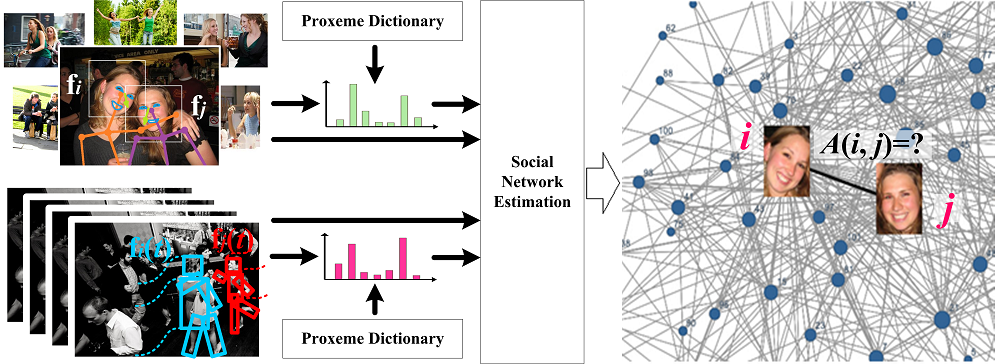
\includegraphics[width=\columnwidth]{intro_2014}
%\end{center}
%\vspace{-0.25in} \caption{\captionsize 
%Social visual analytics: A computational foundation for recovering information from image and video collections about social relationships and social networks through social proxemes. \label{fig:intro}\afterfigspace}
%\end{figure}
%





\comment{related work:
Study of non-verbal communication. Hall describes a set of four categories of inter-personal distances, and later equates the term `proxeme' with the phoneme of language~\cite{Hall}. Birdwhistell defines `kineme' as the minimal unit of an individual's visual expression (body movement, facial expression, or gesture). Kendon talks about interaction units that are space-time structures of \emph{relative} visual expressions, and introduces categories known as `f-formations' (see Fig.~X). We use the phrase proxeme.

"kineme" is "similar to a phoneme because it consists of a group of movements which are not identical, but which may be used interchangeably without affecting social meaning". (Knapp 1972:94-95)

, including areas of proxemics~\cite{hall} and kinesics~\cite{birstwell}. Kendon formalizes this procedure in video as context analysis, can be seen a particular instance of the analytical process of \emph{coding} used for qualitative analysis in social science. In this process, a set of categories are \emph{codes} are produced by experts through repeated observations of videos. rough definition of codes. We seek to automate this process.

Inspired by computational sociology~\cite{hall1974,Kendon1990,Lazer2009,Pantic} where a social interaction is described as a co-occurrence of two or more individual behaviors that are together distinctive in space and time, we will develop new representations of interactions comprised of mixed ensembles of individual behavior descriptors and relative pair-wise behavior descriptors.  Social science also suggests that, in a variety of settings/domains, interactions can be usefully categorized into a manageable number of classes \cite{hall1974,Kendon1990,Hoyle,Tannen,econo_category,Scherr2009}. These classes change from setting to setting, for example, f-formations at a cocktail party \cite{Kendon1990}, or student interactions in a physics tutorial \cite{Scherr2009}. We use "proxemes" to refer to such classes (interaction categories)\footnote{While this term is inspired by \cite{hall1974}, we use it to refer to a larger number and variety of categories in broader settings than those originally considered in \cite{hall1974}}. 
}


%%%%%%%%%%%%%%%%%%%%%%%%%%%%%%%%%%%%%%%%%%%%%%




%Among the large variety of interactions occurring in imagery, there are a few interactions that strongly correlate to social relationships and are informative about social networks\cite{hall1974,Hoyle,Tannen,econo_category,Scherr2009}, and these interactions are referred to as ``proxemes" \cite{hall1974}.  

%, and our preliminary results show that this can provide an attractive balance of discriminative power, robustness, and efficiency.

%\vspace{-0.1in}\item \emph{Learning social interaction categories.} Social science suggests that interactions can often be usefully categorized into a manageable number of classes (e.g.,~\cite{Kendon1990,Hoyle,Tannen,econo_category,Scherr2009}), but discovering these categories is currently an onerous task for human experts that cannot be easily scaled to many different environments or to more than a few participants. To address this, we will develop computational tools for supervised and semi-supervised learning of interaction categories, along with effective and efficient detectors to go with them.

%\vspace{-0.1in}\item \emph{Inferring social networks from visual data.} We will create computational methods for estimating social networks from multiple visual cues, including detected occurrences of social interaction categories. We argue that existing network reconstruction tools are not optimized for visual input, and we propose a new class of techniques to improve performance when: (a) the visual descriptors are derived from diverse sources, are very noisy, and are often missing; (b) the underlying social network contains multiple overlapping communities; and (c) the identities associated with detected and tracked agents are uncertain. 

%\todd{Merge into end of 3.0.} Our research is timely because of maturing technologies for detecting and tracking the faces and bodies of people and recognizing their identities. A variety of serviceable systems exist, and by integrating them one can extract crude but usable descriptors of individual and relative behaviors in the form of positions, trajectories, histograms-of-flow, bags of interest points, and so on. When image quality permits, these can also be augmented with more detailed descriptors computed from head pose and body pose. In any case, with these types of features an image can be abstracted as a noisy collection of positional features, and a video can be abstracted as a noisy collection of space-time features (see Fig.~\ref{fig:intro}). These are the abstractions on which we propose to operate.

%\todd{Merge into end of 3.0.} Our goal is to enable the automatic recovery of useful information about social relationships and the underlying social network using \emph{today's} tools for detection and tracking, with the understanding that our accuracy will automatically increase as these tools continue to evolve. A principal challenge, therefore is to handle the substantial and unavoidable uncertainties caused by false detections, broken tracks, erroneous descriptors, and mis-recognitions, and we seek general methods that can exploit inputs of varying precision. High-quality imagery can provide fine-scale information about expression, while low-quality imagery might provide only coarse estimates of head pose. Our goal is to create general tools that operate in all cases and make use of as much information as is available.


%The proposal is organized as follows. Following a discussion of related work in Section 2, we being our proposed research in Section 3.1 by discussing representations for social interactions and the detection and recognition of an interaction in an image or a long video of a large social gathering. In Section 3.2, we discuss how this technology will  discover and learn salient interaction categories in semi-supervised and unsupervised scenarios, and ho wit will optimize the detection and recognition. Section 3.3 moves on to describe how to infer social network information from interactions that are detected over time and space in large image and video collections, with a focus on robustly associating identities to targets in the images/videos and effectively reconstructing noisy and incomplete multi-view networks. Finally, Section 3.4 describes data collection and challenge problems for evaluation.


%\begin{enumerate}
%\item  Detecting and recognition of interaction categories. Relatively mature in images due to face detection, person detection, and pose estimation.  But largely unsolved in videos. We will address the questions including 1) How do we represent an interaction category? 2) How do we identify in a long video of a large gathering 3) when this interaction occurs, and 4) who it involves? To do so, we will develop approaches to learn effective and efficient interaction detector for  a given set of categories. These socially-salient interaction categories may arise from sociology \cite{Kendon1990,Ekman,Hoyle,Tannen,Goodwin2000,Goldin,Goodwin2007,Kendon2010,Lazer2009}, but this does not scale in novel environments and applications. Therefore, we will develop approaches to learn representations for new categories from image/video collections in a semi-supervised or unsupervised manner.
%\item Inferring social network information from detected interactions. We will design mechanisms by which we distill ties or affinities between social members from multiple heterogeneous visual cues, and in particular accounting for the multi-view effect in a practical social network. To achieve robustness, our research will especially focus on noise-resilient methods for mapping image targets to the identities of the members, as well as novel algorithms to the case of incomplete and noisy outputs from the social network estimator due to various types of imperfection incurred from missed detections; mis-classified interactions, and a large fraction of missing observations.
%\item Data collections and challenge problems. We will collect datasets to evaluate our methods and design challenge problems to engage our colleagues in this research agenda. To do this, we will address the challenges of enabling reproducible research while preserving privacy.
%\end{enumerate}


